% 13
\begin{frame}{Sterowanie impedancyjne napędu}
\begin{columns}[T,onlytextwidth]
\column{0.56\textwidth}
\begin{block}{Idea: wirtualna sprężyna i tłumik}
\[
\tau = K_p(q_d-q) + K_d(\dot q_d-\dot q) + \tau_{\mathrm{ff}}
\]
\end{block}
\begin{itemize}
  \item $K_p$ - wzmocnienie części proporcjonalnej: „sztywność”.
  \item $K_d$ - wzmocnienie części zależnej od prędkości: „tłumienie”.
  \item $\tau_{\mathrm{ff}}$ - moment wyprzedzający, zadany z wyższego poziomu sterowania.
\end{itemize}
\column{0.40\textwidth}
\begin{center}
\begin{tikzpicture}[node distance=0.55cm,>=Latex]
  \tikzstyle{box}=[draw,rounded corners=2pt,fill=blue!6,minimum width=2.8cm,minimum height=0.65cm,align=center,font=\scriptsize]
  \node[box] (ref) {pozycja i prędkość\\zadana};
  \node[box,below=of ref] (law) {$K_p e_q + K_d e_{\dot q}$\\$+\;\tau_{\mathrm{ff}}$};
  \node[box,below=of law] (motor) {sterownik prądu\\i silnik};
  \node[box,below=of motor] (enc) {enkoder};
  \draw[->,thick] (ref)--(law);
  \draw[->,thick] (law)--node[right,font=\scriptsize] {$\tau$} (motor);
  \draw[->,thick] (motor)--(enc);
  \draw[->,thick] (enc.west) .. controls +(-0.9,0) and +(-0.9,0) .. (law.west);
\end{tikzpicture}
\end{center}
\end{columns}
\source{Załączony PDF wskazuje tryb impedancyjny sterowników napędów oraz komunikację ROS 2/CAN.}
\note{Ten slajd buduje most do sprzętu: wyższa warstwa nie musi zawsze wysyłać surowych momentów. Może zadawać pozycje, prędkości, sztywności i feed-forward, jeśli sterownik napędu to obsługuje.}
\end{frame}

% 14
\begin{frame}[fragile]{„Model” w praktyce: interfejs, nie dogmat}
\begin{columns}[T,onlytextwidth]
\column{0.51\textwidth}
\begin{lstlisting}[style=pseudocode,basicstyle=\ttfamily\scriptsize]
state = read_sensors()
q  = state.joint_position
dq = state.joint_velocity

foot = model.foot_position(q)
J    = model.foot_jacobian(q)
h    = model.safety_margins(q, dq)
\end{lstlisting}
\column{0.45\textwidth}
\small
\begin{itemize}
  \item Model może być analityczny, numeryczny lub częściowo zidentyfikowany.
  \item Najważniejsze pytanie: \key{czy przewiduje właściwe ryzyka?}
  \item Na początku wystarczą kinematyka, ograniczenia, margines osobliwości i prosta dynamika.
\end{itemize}
\end{columns}
\note{To dobry slajd do rozbrojenia obawy, że model musi być idealny. Sterowanie predykcyjne potrzebuje modelu użytecznego dla horyzontu predykcji, nie kompletnego cyfrowego bliźniaka.}
\end{frame}

% 15
\begin{frame}{MPC: Model Predictive Control w jednym zdaniu}
\begin{block}{Definicja robocza}
\key{Model Predictive Control (MPC)}, czyli sterowanie predykcyjne oparte na modelu, wybiera teraz takie sterowanie, które według modelu da najlepszy i bezpieczny ruch w najbliższej przyszłości.
\end{block}
\vspace{-0.2em}
\[
\begin{aligned}
\min_{u_0,\ldots,u_{N-1}}\quad
&\sum_{k=0}^{N-1} \ell(x_k,u_k)+\ell_N(x_N)\\
\text{przy ograniczeniach}\quad
&x_{k+1}=f(x_k,u_k),\\
&x_k\in\mathcal X,\qquad u_k\in\mathcal U.
\end{aligned}
\]
\begin{itemize}
  \item $x_k$ - przewidywany stan, $u_k$ - sterowanie, $N$ - horyzont predykcji.
  \item Wykonujemy tylko pierwszy krok, potem mierzymy stan i rozwiązujemy problem ponownie.
\end{itemize}
\note{To slajd, który warto zostawić dokładnie w tej roli: definicja i wzór w jednym miejscu. Nie należy rozwlekać tu teorii optymalizacji.}
\end{frame}

% 16
\begin{frame}[fragile]{MPC jako przesuwający się horyzont}
\begin{columns}[T,onlytextwidth]
\column{0.55\textwidth}
\begin{lstlisting}[style=pseudocode,basicstyle=\ttfamily\scriptsize]
repeat at control rate:
    measure state x
    predict with model f
    reject infeasible plans
    minimize tracking + effort + risk
    apply only control u_0
\end{lstlisting}
\column{0.41\textwidth}
\begin{center}
\begin{tikzpicture}[>=Latex,scale=0.95]
  \foreach \i in {0,...,5} {
    \draw[fill=blue!5] (0.62*\i,0) circle (0.08);
  }
  \draw[->,thick,pwrblue] (0,0)--(3.2,0);
  \draw[thick,warn] (0,0.35)--(3.1,0.35);
  \node[font=\scriptsize] at (1.55,0.68) {predykcja};
  \draw[->,very thick,safe] (0,-0.35)--(0.62,-0.35);
  \node[font=\scriptsize,align=center] at (1.45,-0.68) {wykonujemy tylko\\pierwszy krok};
\end{tikzpicture}
\end{center}
\begin{itemize}
  \item Plan jest stale poprawiany po nowych pomiarach.
  \item Ograniczenia są częścią zadania, nie dopiskiem po fakcie.
\end{itemize}
\end{columns}
\note{Dla laików najważniejsza jest intuicja: MPC nie układa pełnej trasy raz na zawsze. Cały czas planuje krótki horyzont i wykonuje pierwszy element planu.}
\end{frame}

% 17
\begin{frame}{Najprostszy demonstrator MPC dla jednej nogi}
\begin{columns}[T,onlytextwidth]
\column{0.46\textwidth}
\begin{block}{Model kinematyczny użyty w kodzie}
\[
x_k=q_k,\qquad u_k=\dot q_k,
\]
\[
q_{k+1}=q_k+\Delta t\,u_k.
\]
\end{block}
\begin{itemize}
  \item Cel: przesunąć stopę do zadanego punktu.
  \item Ograniczenia: kąty, prędkości, rozstaw boczny i odległość od przełączenia czworoboku.
\end{itemize}
\column{0.50\textwidth}
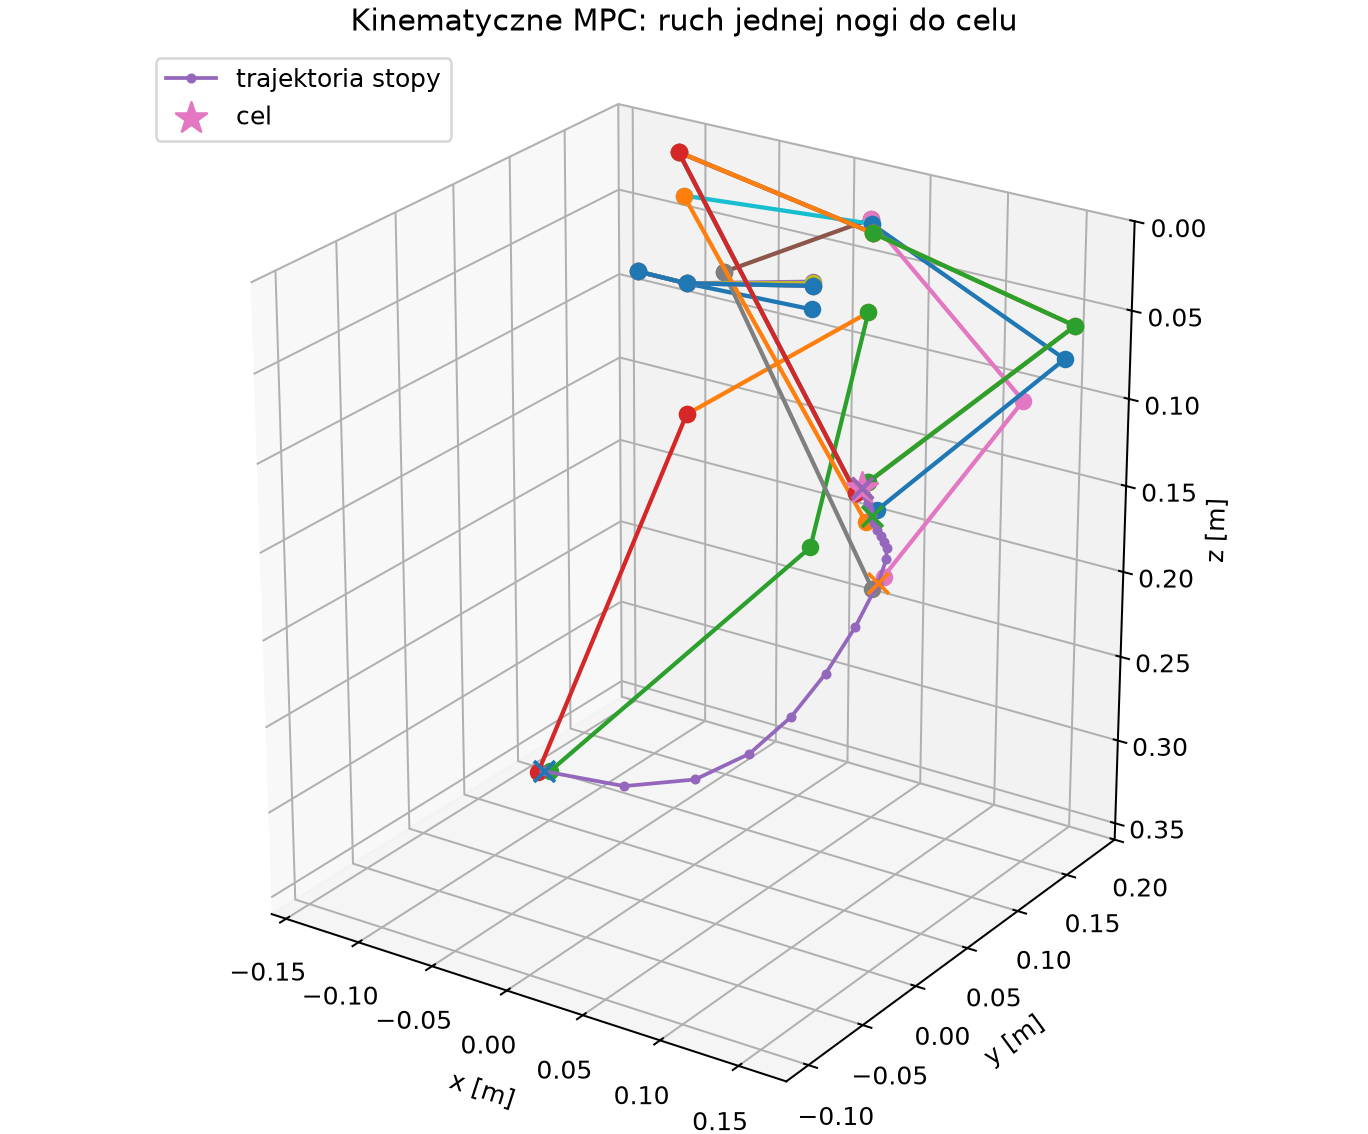
\includegraphics[width=\linewidth,height=0.55\textheight,keepaspectratio]{figures/mpc_leg_trajectory.png}
\end{columns}
\note{Należy uczciwie powiedzieć, że demonstrator steruje prędkościami przegubów. Model momentowy pojawia się dopiero jako następny etap projektu i w appendixie.}
\end{frame}

% 18
\begin{frame}{Funkcja kosztu i stan demonstratora}
\begin{columns}[T,onlytextwidth]
\column{0.52\textwidth}
\small
\[
\begin{aligned}
J ={}& w_p\|p_F-p_F^{\mathrm{ref}}\|^2
 + w_q\|q-q_{\mathrm{nom}}\|^2\\
&+ w_u\|\dot q\|^2
 + w_{\Delta u}\|\Delta\dot q\|^2.
\end{aligned}
\]
\begin{itemize}
  \item $w_p$: dokładność położenia stopy.
  \item $w_q$: preferowana, odzyskiwalna postawa.
  \item $w_u$: umiarkowane prędkości napędów.
  \item $w_{\Delta u}$: płynne zmiany sterowania.
\end{itemize}
\column{0.44\textwidth}
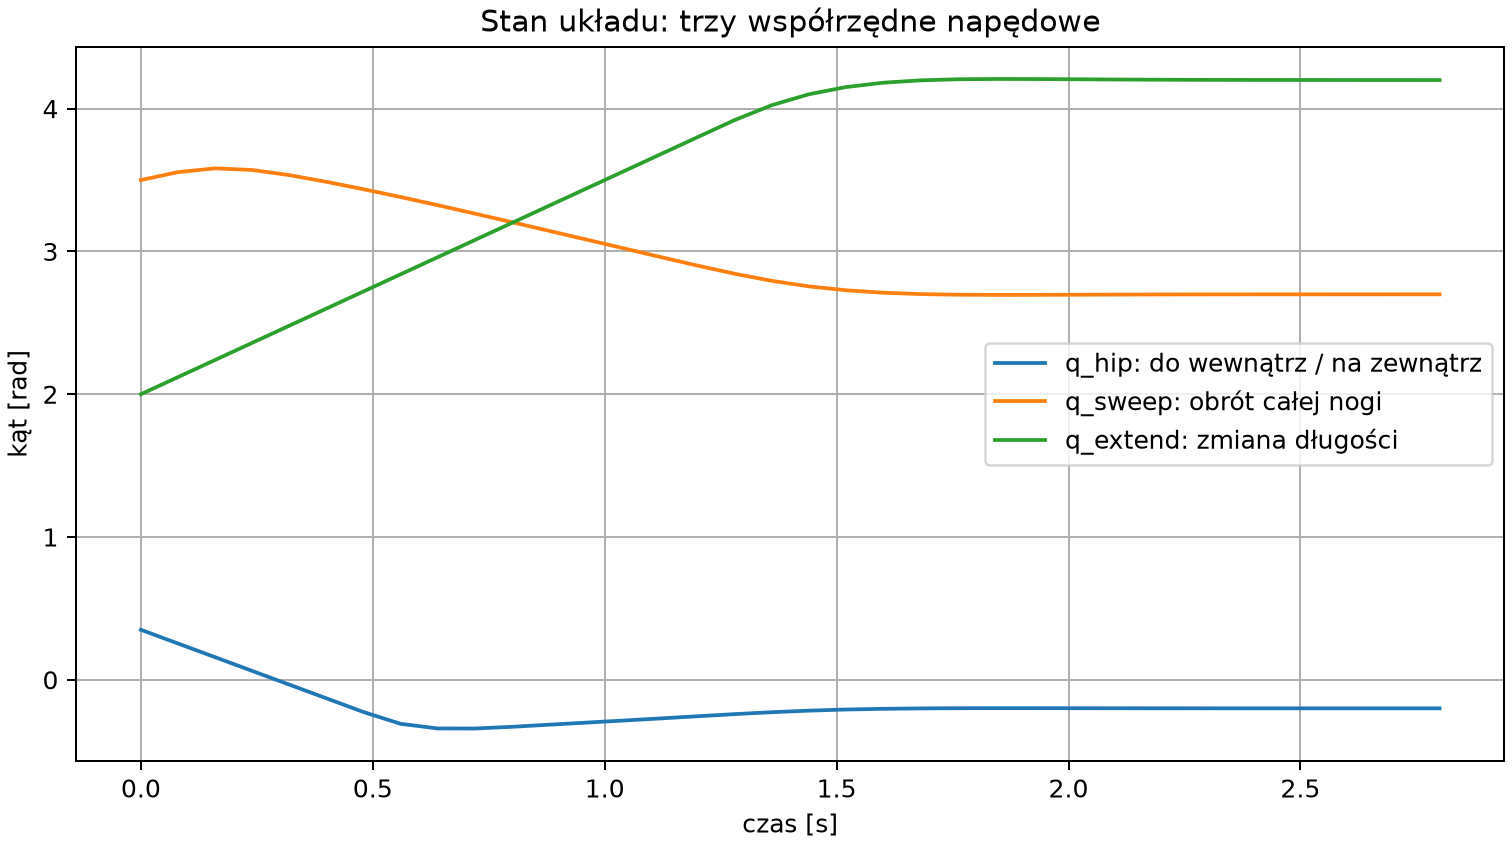
\includegraphics[width=\linewidth,height=0.50\textheight,keepaspectratio]{figures/mpc_joint_states.png}
\end{columns}
\begin{block}{Następny poziom}
Po identyfikacji dynamiki wejście $u=\dot q$ można zastąpić momentem $u=\tau$.
\end{block}
\note{Ten slajd usuwa niespójność między kodem a wcześniejszą wersją prezentacji, która opisywała od razu regulator momentowy.}
\end{frame}
